\section{Auswertung}
\subsection{Energiekalibration}
\begin{itemize}
	\item Spektrum geplottet, Counts gegen Channel
	\item Errorbars?
	\item Peaks finden lassen, Peaks markiert
	\item Literaturwerte Energien rausgesucht mit mind. 1\% Emissionswahrscheinlichkeit (Quelle %http://www.nucleide.org/DDEP_WG/Nuclides/Eu-152_tables.pdf 2019-12-11, 22:35)
	\item Spektrallinien $E$ normiert mit dem größten Wert der Energie: $\frac{E}{max(E)}$
	\item Channel normiert mit dem letzten Peak $\frac{channel}{max(channel)}$
	\item Daten mit normierter x-Achse geplottet: norm(E)-0-Diagramm, norm(channel)-Count-Diagramm
	\item Nicht vorhandene Spektrallinien aus E und doppelte aus Peaks entfernt
	\item Peak-Channel gegen Energien geplottet, Fit:
\end{itemize}
\begin{equation*}
	E = m \cdot \text{Channel} + n
\end{equation*}
\begin{align*}
	m = \SI{0.20726(4)}{\kilo \electronvolt \per Channel} && n = \SI{-1.22(17)}{\kilo \electronvolt}
\end{align*}

\begin{table}[h!]
  \centering
  \caption{Parameter zu allen vermessenen Peaks des $^{152}\symup{Eu}$-Spektrums.}
  \label{tab:eu_peaks}
  \begin{tabular}{ r  r  r  r  r  r  }
    \bottomrule
            Peak & Channel(Peak)  & Counts  &  $E_{\gamma}$ / keV \cite{nucleide} & rel. Channel                                       & rel. Energie  \\ % & $a$                              &      $\mu$                         & $\sigma$                         & $b$                              \\
                 &                &         &                                     & $\frac{\text{Channel}}{\text{Channel(Peak 9)}}$    & $\frac{E_{\gamma}}{E_{\gamma}\text{(Peak 9)}}$ \\ % & $a$                              &      $\mu$                         & $\sigma$                         & $b$                              \\
    \midrule
            0    &  594           &  1219   &  $\SI{121.7817}{\nothing}$          & 0,087                                              & 0,087 \\
            1    &  1187          &  196    &  $\SI{244.6974}{\nothing}$          & 0,175                                              & 0,174 \\
            2    &  1667          &  372    &  $\SI{344.2785}{\nothing}$          & 0,245                                              & 0,245 \\
            3    &  1988          &  42     &  $\SI{411.1165}{\nothing}$          & 0,292                                              & 0,292 \\
            4    &  2149          &  43     &  $\SI{ 443.965}{\nothing}$          & 0,316                                              & 0,315 \\
            5    &  3765          &  66     &  $\SI{778.9045}{\nothing}$          & 0,554                                              & 0,553 \\
            6    &  4655          &  41     &  $\SI{ 964.079}{\nothing}$          & 0,685                                              & 0,685 \\
            7    &  5245          &  32     &  $\SI{1085.837}{\nothing}$          & 0,771                                              & 0,771 \\
            8    &  5371          &  33     &  $\SI{1112.076}{\nothing}$          & 0,790                                              & 0,790 \\
            9    &  6801          &  37     &  $\SI{1408.013}{\nothing}$          & 1,0                                                & 1,0 \\
    \toprule
  \end{tabular}
\end{table}
%                                &  \scriptsize{$\sfrac{mN}{sm}{a}$}            &  \scriptsize{$\sfrac{mN}{m}{a}$}          &  \scriptsize{$\sfrac{mN}{m}{a}$} &  \scriptsize{$\sfrac{mN}{m}{a}$} & \scriptsize{$\sfrac{mN}{m}{a}$} \\ \hline \hline
%    \rowcolor{Lightgray} \multicolumn{7}{|c|}{Referenzen}\\ \hline
%        \multirow{2}{*}{\ce{C3F8}}  & 1  & $\SI{ 1.3396 \pm 0.0202 e-3}{\nothing}{a}$  &  $\SI{ -0.5415 \pm 0.0558 }{\nothing} $  &  $\SI{ 0.00 }{\nothing}{a}$      &  $\SI{ 5.72 }{\nothing}{a}$   & $\SI{ 5.72 }{\nothing}{a}$    \\


\begin{figure}[h!]
  \centering
  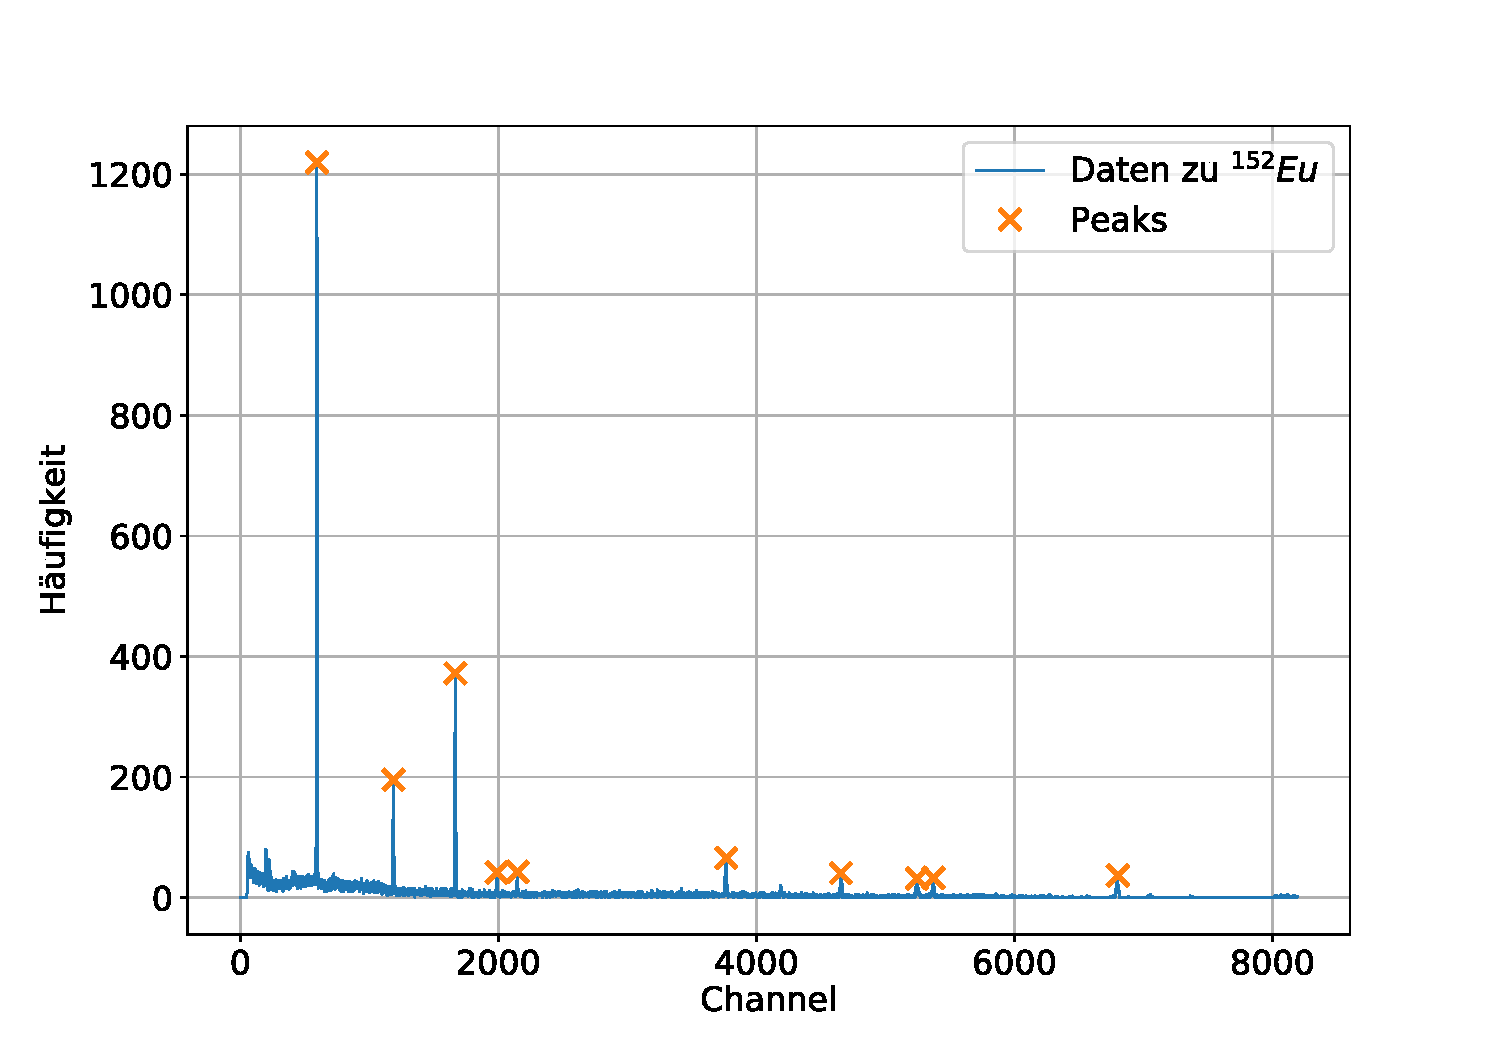
\includegraphics[width=\textwidth]{content/images/spektrum_europium.pdf}
  \caption{Das aufgenommene Spektrum von $^{152}Eu$ mit eingezeichneten Peaks.}
  \label{fig:eu_spect}
\end{figure}

\begin{figure}[h!]
  \centering
  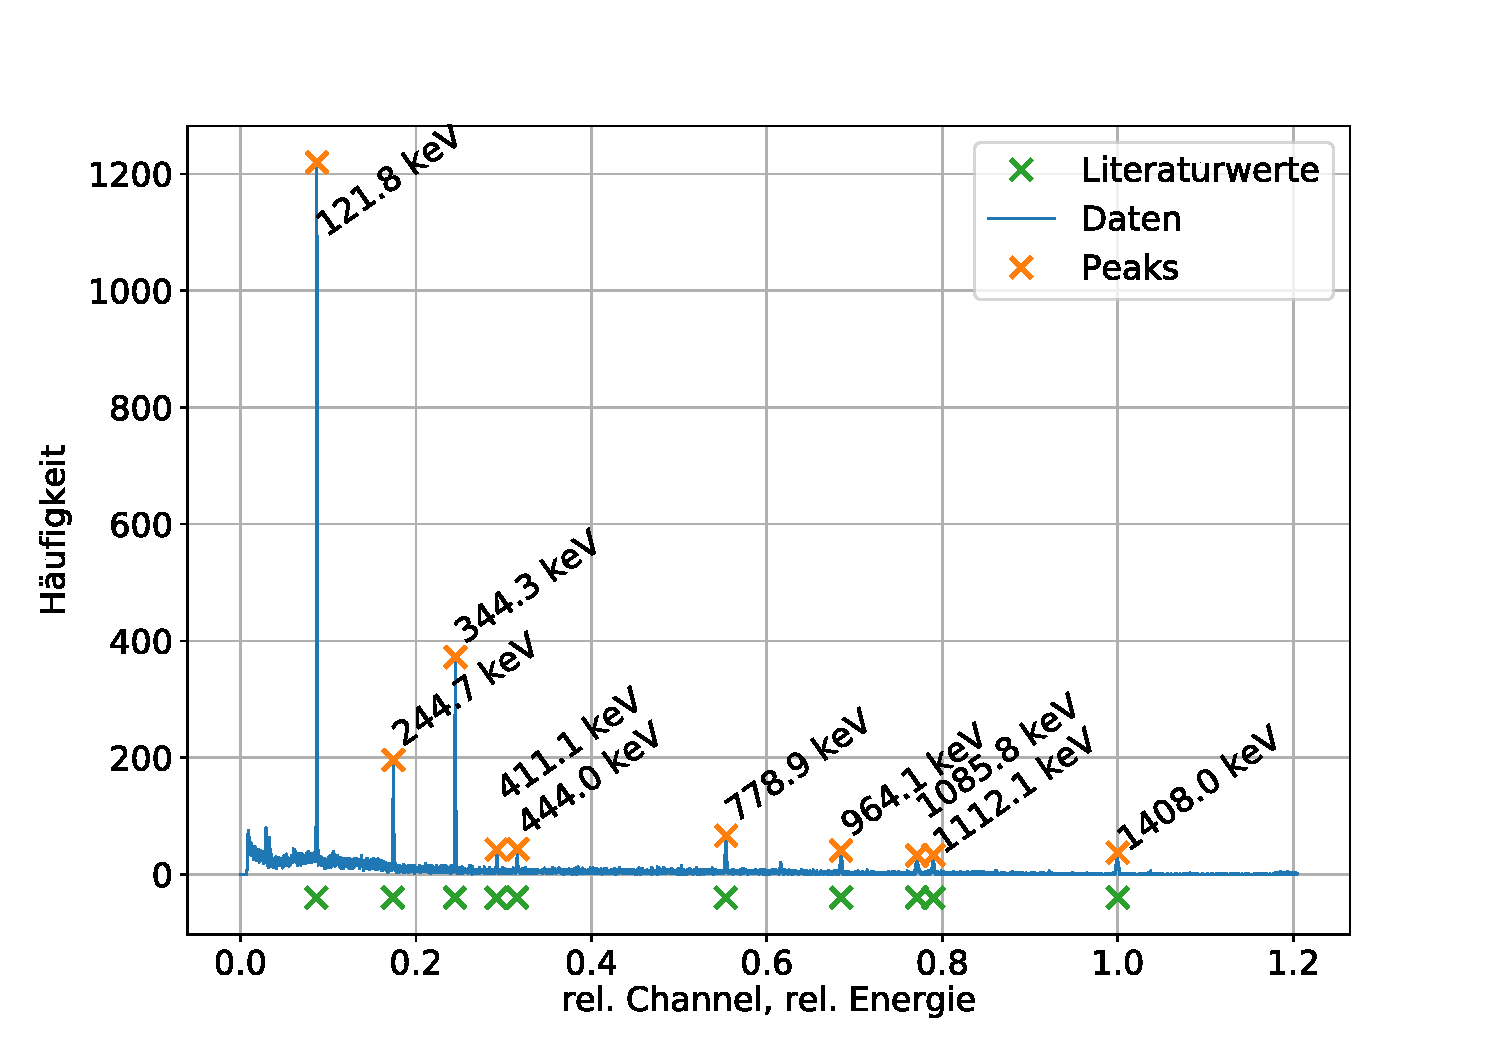
\includegraphics[width=\textwidth]{content/images/spektrum_europium_kali.pdf}
  \caption{Das aufgenommene Spektrum von $^{152}Eu$ mit eingezeichneten Peaks und den zugehörigen Literaturwerten nach \cite{nucleide}.}
  \label{fig:eu_spect_kali}
\end{figure}

\begin{figure}[h!]
  \centering
  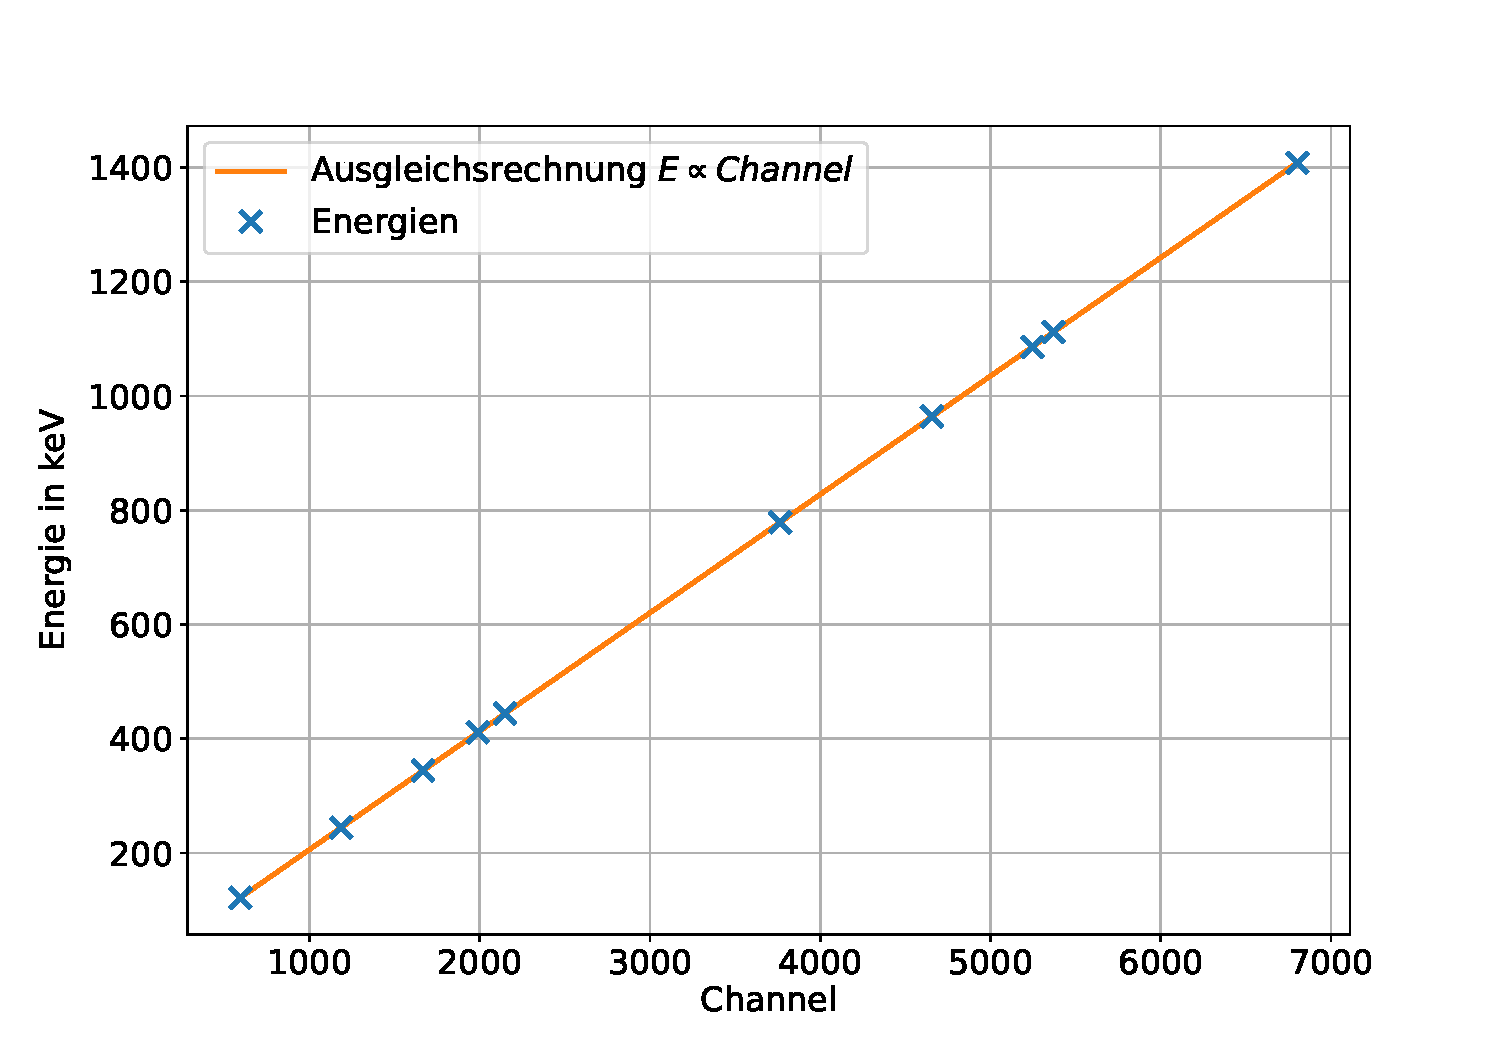
\includegraphics[width=\textwidth]{content/images/kalibration.pdf}
  \caption{Ausgleichsrechnung zur Kalibration mithilfe des $^{152}Eu$-Spektrums.}
  \label{fig:kali}
\end{figure}

\FloatBarrier
\subsection{Vollenergienachweiswahrscheinlichkeit}
mit $t = \SI{605484000 (54000)}{s}$
und $T_{\sfrac{1}{2}} = \SI{426.7 (5) e+06}{s}$ \cite{nucleide}
\begin{equation}
	A = A_{0} \exp{\left( - \frac{\ln{(2))}}{T_{\sfrac{1}{2}}} t \right)} = \SI{1545(29)}{\per \second}
	\label{result:aktivität}
\end{equation}
mit $r=\SI{22.5e-03}{m}$
und $h = \SI{80e-03}{m}$
\begin{align*}
	\frac{r}{h} = \tan{( \varphi / 2 )} \Leftrightarrow \varphi = 2 \arctan{(\frac{r}{h})} \\
	\frac{\Omega}{4 \pi} = \sin^2{\frac{\varphi}{2 \cdot 4}} =  \sin^2{ \left( \frac{1}{4} \arctan{(r/h)} \right)} = \SI{0.0069}{sr}
	\label{result:raumwinkel}
\end{align*}
und
\begin{equation}
	Q = \frac{4 \pi}{\Omega} \frac{N_{\text{Peakinhalt}}}{ A T P_{E_{\gamma}}}
\end{equation}

\begin{figure}[h!]
  \centering
  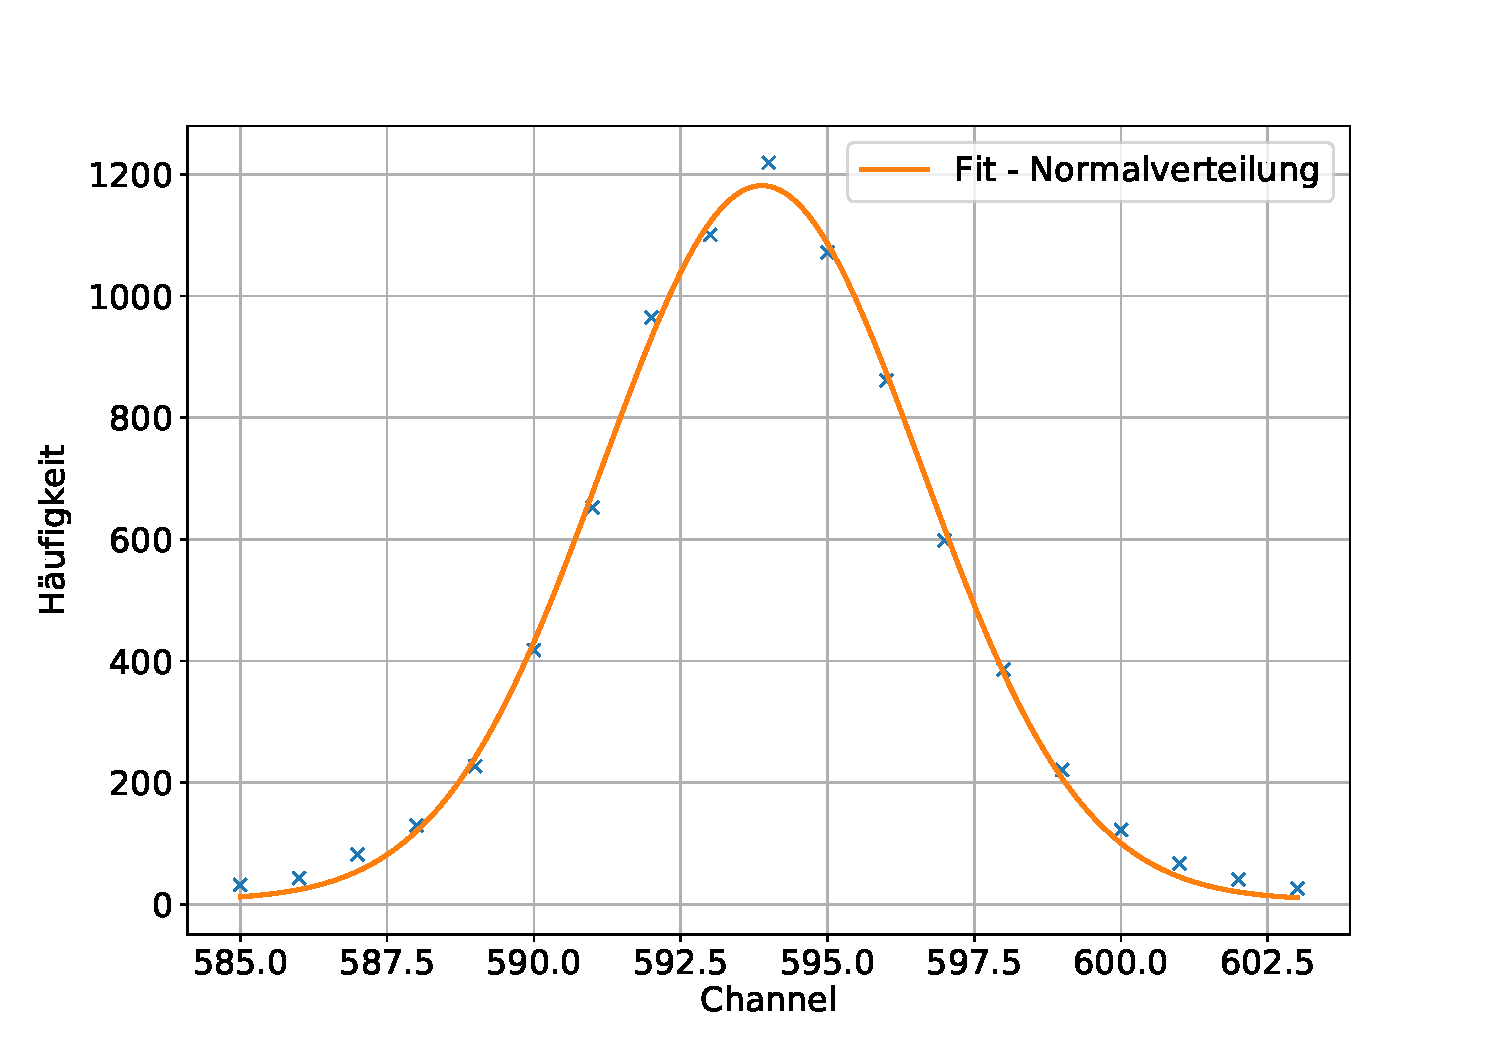
\includegraphics[width=\textwidth]{content/images/einzelnergaussfit_0.pdf}
  \caption{Vergrößerung des ersten Peaks mit Ausgleichsfunktion einer Gaußkurve zur Veranschaulichung der Gaußpeaks.}
  \label{fig:vw}
\end{figure}

\begin{table}[h!]
  \centering
  \caption{Parameter zur Berechnung der Vollenergienachweiswahrscheinlichkeit anhand eines $^{152}\symup{Eu}$-Spektrums. Weitere verwendete Größen sind: \\ $A=\SI{1545(29)}{\per \second}$, $\frac{\Omega}{4 \pi} = \SI{0.0069}{sr}$, $T=\SI{2134}{s}$.}
  \label{tab:vw}
  \begin{tabular}{ r  r  r  r  r  r  }
    \bottomrule
              $E_{\gamma}$ / keV \cite{nucleide} & $P$ \cite{nucleide}   & $P_{\text{Peakinhalt}}$    & Q in $10^{-3}$            \\ % & $a$                              &      $\mu$                         & $\sigma$                         & $b$                              \\
    \midrule
                $\SI{121.7817}{\nothing}$        & $\SI{28.41}{\nothing}$& $\SI{8233 (91)}{\nothing}$ & $\SI{12.70 (24)}{\nothing}$            \\ % & $\SI{54643  (699)}{a}$  & $\SI{593.88 (0.02}}{a}$      & $\SI{2.72080278 (0.02096791)}{a}$  & $\SI{6.65464370 (0.155416486)}{a}$ \\
                $\SI{244.6974}{\nothing}$        & $\SI{ 7.55}{\nothing}$& $\SI{1515 (39)}{\nothing}$ & $\SI{ 8.79 (16)}{\nothing}$            \\ % & $\SI{10583 (1892)}{a}$  & $\SI{1186.58105 (0.33278)}{a}$       & $\SI{3.08985566 (0.33289872)}{a}$  & $\SI{7.46589080 (0.347744578)}{a}$ \\
                $\SI{344.2785}{\nothing}$        & $\SI{26.59}{\nothing}$& $\SI{3152 (56)}{\nothing}$ & $\SI{ 5.19 (10)}{\nothing}$            \\ % & $\SI{25365 (2038)}{a}$  & $\SI{1666.69026 (0.16131)}{a}$       & $\SI{3.33202744 (0.16137103)}{a}$  & $\SI{7.26196957 (0.334424003)}{a}$ \\
                $\SI{411.1165}{\nothing}$        & $\SI{2.238}{\nothing}$& $\SI{ 324 (18)}{\nothing}$ & $\SI{ 6.34 (12)}{\nothing}$            \\ % & $\SI{ 1320 (1390)}{a}$  & $\SI{1989.13968353 (1.58221965)}{a}$ & $\SI{2.49555989 (1.58264810)}{a}$  & $\SI{7.60693051 (0.351207638)}{a}$ \\
                $\SI{ 443.965}{\nothing}$        & $\SI{ 2.80}{\nothing}$& $\SI{ 367 (19)}{\nothing}$ & $\SI{ 5.74 (11)}{\nothing}$            \\ % & $\SI{ 1839 (1909)}{a}$  & $\SI{2147.41246865 (1.92603485)}{a}$ & $\SI{3.08211825 (1.92667938)}{a}$  & $\SI{7.60363599 (0.351271659)}{a}$ \\
                $\SI{778.9045}{\nothing}$        & $\SI{12.97}{\nothing}$& $\SI{ 741 (27)}{\nothing}$ & $\SI{ 2.50  (5)}{\nothing}$            \\ % & $\SI{ 6632 (3679)}{a}$  & $\SI{3763.60345 (1.60581703)}{a}$    & $\SI{4.79839449 (1.60665042)}{a}$  & $\SI{7.56537596 (0.351196062)}{a}$ \\
                $\SI{ 964.079}{\nothing}$        & $\SI{14.50}{\nothing}$& $\SI{ 596 (24)}{\nothing}$ & $\SI{ 1.80 (33)}{\nothing}$            \\ % & $\SI{ 5190 (4028)}{a}$  & $\SI{4656.71298 (2.39004332)}{a}$    & $\SI{5.10185800 (2.39136059)}{a}$  & $\SI{7.58314830 (0.351416184)}{a}$ \\
                $\SI{1085.837}{\nothing}$        & $\SI{10.13}{\nothing}$& $\SI{ 403 (20)}{\nothing}$ & $\SI{ 1.74 (32)}{\nothing}$            \\ % & $\SI{ 2217 (3342)}{a}$  & $\SI{5244.21808 (4.04291370)}{a}$    & $\SI{4.46961617 (4.04488016)}{a}$  & $\SI{7.60853282 (0.351488937)}{a}$ \\
                $\SI{1112.076}{\nothing}$        & $\SI{13.41}{\nothing}$& $\SI{ 502 (22)}{\nothing}$ & $\SI{ 1.64 (30)}{\nothing}$            \\ % & $\SI{ 3576 (3677)}{a}$  & $\SI{5370.46910 (2.93022325)}{a}$    & $\SI{4.74729689 (2.93174255)}{a}$  & $\SI{7.59600458 (0.351461227)}{a}$ \\
                $\SI{1408.013}{\nothing}$        & $\SI{20.85}{\nothing}$& $\SI{ 586 (24)}{\nothing}$ & $\SI{ 1.23 (23)}{\nothing}$            \\ % & $\SI{ 5304 (5433)}{a}$  & $\SI{6798.07269 (4)}{a}$    & $\SI{6.16476521 (3.79392683)}{a}$  & $\SI{7.59078829 (0.351623258)}{a}$ \\
    \toprule
  \end{tabular}
\end{table}
%                                &  \scriptsize{$\sfrac{mN}{sm}{a}$}            &  \scriptsize{$\sfrac{mN}{m}{a}$}          &  \scriptsize{$\sfrac{mN}{m}{a}$} &  \scriptsize{$\sfrac{mN}{m}{a}$} & \scriptsize{$\sfrac{mN}{m}{a}$} \\ \hline \hline
%    \rowcolor{Lightgray} \multicolumn{7}{|c|}{Referenzen}\\ \hline
%        \multirow{2}{*}{\ce{C3F8}}  & 1  & $\SI{ 1.3396 \pm 0.0202 e-3}{\nothing}{a}$  &  $\SI{ -0.5415 \pm 0.0558 }{\nothing} $  &  $\SI{ 0.00 }{\nothing}{a}$      &  $\SI{ 5.72 }{\nothing}{a}$   & $\SI{ 5.72 }{\nothing}{a}$    \\


\begin{itemize}
	\item Unterteilung der Daten in die Abschnitte um die Peaks (channel und counts werden passend abgeschnitten)
	\item Über die Peaks wird eine Gaußkurve gelegt $f (x) = \frac{a}{\sqrt{2 \pi \sigma^2}} \exp{\left( - \frac{(x-\mu)^2}{2 \sigma^2} \right)}+b$
	\item Klappt bei den meisten Peaks ganz gut, aber manchmal ist der Fehler des Parameters $a$ größer als a :|
	\item Alternative für Inhalt: Aufsummation der Counts in den jeweiligen Intervallen, Fehler über den Poisson-Fehler ($N \pm \sqrt{N}$)
	\item $Q$ berechnet mit $A$ aus \eqref{result:aktivität}, $\sfrac{\Omega}{4 \pi}$ aus \eqref{result:raumwinkel},
	gesamte Messzeit $T=\SI{2134}{s}$, Emissionswahrscheinlichkeit $P_{E_{\gamma}}$ aus \cite{nucleide}, Peakinhalt $N_{\text{Peakinhalt}}$
	\item $Q$ gegen $E$ aufgetragen, $Q=a E^{b} + c$, Parameter:
\end{itemize}
\begin{align*}
	a = \SI{0.113 (55)}{\frac{1}{J}}, && b = \SI{-0.36 (17)}{\nothing}, && c = \SI{-0.0077 (59)}{\nothing}
\end{align*}

\begin{figure}[h!]
  \centering
  \includegraphics[width=\textwidth]{content/images/vollenergienachweiswahrscheinlichkeit.pdf}
  \caption{Ausgleichsrechnung zur Bestimmung der Vollenergienachweiswahrscheinlichkeit $Q$.
  Die Fehlerbereiche verschwinden hinter den Datenpunkten und sind zur Übersichtlichkeit nicht aufgeführt.}
  \label{fig:vw}
\end{figure}

\FloatBarrier
\subsection{Monoenergetisches Spektrum Cäsium}
Suche
\begin{itemize}
	\item Energie des Strahlers (Photo-Energie -> Gauss fitten? mu entspricht dann dem Channel und der Channel einer Energie)
	\item Fit:
	\begin{equation*}
		f(x) = \frac{a}{\sqrt{2 \pi \sigma^2}} \, \exp{\left( - \frac{(x-\mu)^2}{2 \sigma^2} \right)} + b
	\end{equation*}
	\item Parameter
	\begin{align*}
		\mu = \SI{3196.29 (3)}{\nothing} && \sigma = \SI{4.35 (3)}{\nothing} && a = \SI{9011 (44)}{\nothing} && b = \SI{6.1 (1)}{\nothing}
	\end{align*}
	\item Halbwertsbreite fitten
	\item Zehntelwertsbreite fitten, $FWHM/FWTM(Theorie) = 0.549$, in den Daten: $FWHM/FWTM = 0.526$
	\item
	\begin{align*}
		FWHM = 10 && FWTM = 19
	\end{align*}
	\item Comptonkante ausmessen
	\item Rückstreulinie ausmessen
	\item Inhalte des Peaks und des Compton-Kontinuums ausmessen (aufsummieren, aaaaber... Anleitung!)
\end{itemize}
